\documentclass{article}
\usepackage[utf8]{inputenc}
\usepackage[T1]{fontenc}
\usepackage{graphicx}
\usepackage{hyperref}
\usepackage{geometry}
\geometry{margin=1in}

\title{MIDWIFERY and OBSTETRICS (Plate CCCXLVII)}
\date{Encyclopaedia Britannica (1771)}

\begin{document}
\maketitle

\section*{Historical source}
\textbf{Entry ID:} \texttt{entry-britannica-volume-191689065-row-1400-1400} \\
\textbf{Volume ID:} 191689065 \\
\textbf{Character Count:} 1194

\subsection*{Extracted Text}
MIDWIFERY PLATE CCCXLVII.
Fig. 1.
Fig. 2.
Fig. 3.

[HISTORICAL COPPERPLATE ENGRAVING: MIDWIFERY and OBSTETRICS (Plate CCCXLVII)]
Category: Medical Anatomy and Obstetrics
Visual Description: Classical obstetrical copperplate engraving illustrating fetal presentation, pelvic anatomy, and 18th-century obstetrical forceps. Demonstrates William Smellie's obstetrical mechanisms and surgical instruments designed to assist difficult child deliveries.

[Nemotron Super VL Analysis]: The visible headings include "MIDWIFERY," "PLATE CCCXLVII," and labels for "Fig. 1" through "Fig. 4." The engraving displays anatomical diagrams related to childbirth, with Figure 1 depicting the placenta and umbilical cord, while Figures 2 through 4 show fetuses positioned within the uterus and pelvic cavity.
Identified Engraved Figures:
  * Fig. 1: Normal vertex presentation of infant in anatomical pelvis
  * Fig. 2: Breech presentation and obstetrical maneuvers
  * Fig. 3: Curved obstetrical forceps with leather-covered blades
  * Fig. 4: Transverse lie presentation and uterine anatomy
Related Scientific Subjects: Obstetrics, Obstetrical forceps, William Smellie (obstetrician), Pelvic anatomy, Childbirth

\subsection*{Matched Wikipedia Article}
\textbf{Title:} Midwife \\
\textbf{Page ID:} 47456362 \\
\textbf{Revision ID:} 1350826529 \\
\textbf{URL:} \url{https://en.wikipedia.org/wiki/Midwife}


\section*{Source record}
\begin{itemize}
\item \textbf{Dataset:} \texttt{NationalLibraryOfScotland/encyclopaedia\_britannica\_illustrated}
\item \textbf{Dataset Revision:} \texttt{309f765b1ecc83e0a7f7762e44b4a927a7555443}
\item \textbf{Page ID:} \texttt{britannica:309f765b1ecc83e0a7f7762e44b4a927a7555443:train:1400} \\
  \textbf{Filename:} \texttt{page-1400-2d754e996979.jpg} \\
  \textbf{Row Index:} 1400 \\
  \textbf{SHA256:} \texttt{2d754e996979c664...}
\end{itemize}

\begin{figure}[h]
\centering
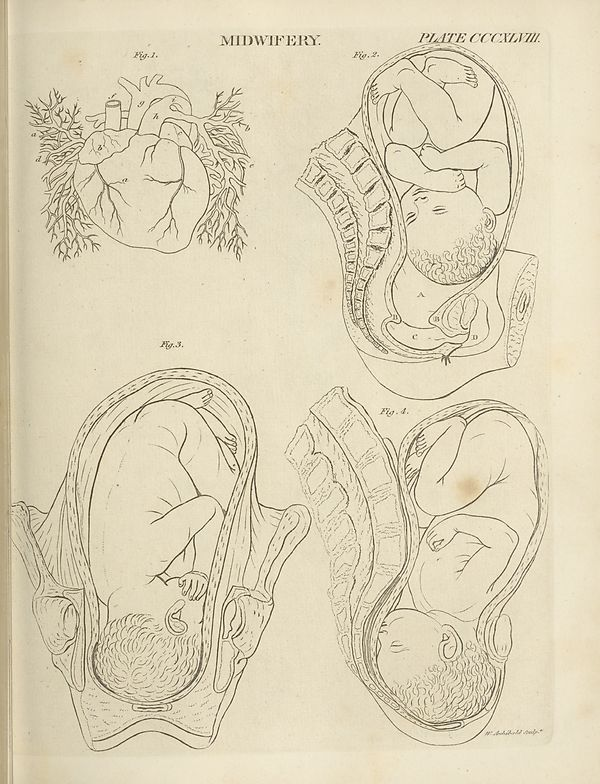
\includegraphics[width=0.85\textwidth]{../scans/page-1400-2d754e996979.jpg}
\caption*{Source scan: \texttt{page-1400-2d754e996979.jpg}}
\end{figure}

\end{document}
